% Svolgimento: prova del 14/09/2026, esercizio 2 -- distribuzione del numero di Mach in un ugello (schlieren).
% Numeri e figure: calcoli.py (stessa cartella). Compilare con: latexmk -pdf svolgimento.tex

\documentclass[11pt,a4paper]{article}

\usepackage[T1]{fontenc}
\usepackage[utf8]{inputenc}
\usepackage[italian]{babel}
\usepackage{amsmath,amssymb}
\usepackage[a4paper,margin=2.5cm]{geometry}
\usepackage{array}
\usepackage{siunitx}
\usepackage{booktabs}
\usepackage{graphicx}
\usepackage{float}
\usepackage{caption}
\usepackage{hyperref}

\hypersetup{hidelinks}
\setlength{\parindent}{0pt}
\setlength{\parskip}{4pt}
\allowdisplaybreaks
\graphicspath{{figure/}}
\sisetup{output-decimal-marker={,}, group-separator={\,}, per-mode=symbol,
         exponent-product=\cdot, range-phrase={\text{--}}}

\newcommand{\Cp}{C^{+}}
\newcommand{\Cm}{C^{-}}

\title{Gasdinamica -- Prova del 14/09/2026, esercizio 2\\[2pt]
\large Distribuzione del numero di Mach in un ugello a valle della gola}
\author{}
\date{}

\begin{document}
\maketitle

\section*{Traccia}
\emph{Stimare la distribuzione del numero di Mach nell'ugello a valle della gola} (Determine the Mach number
distribution in the nozzle downstream of the throat). La traccia è accompagnata da una visualizzazione schlieren
dell'ugello (fig.~\ref{fig:ann}).

%==============================================================================
\section{Lettura del testo e dell'immagine}
La schlieren mostra, attraverso una finestra circolare, la regione di gola di un ugello piano
convergente--divergente. I blocchi neri in alto e in basso sono le pareti; la sezione più stretta è in
corrispondenza dei due fori, che segnano la \textbf{gola}, e la corrente va da sinistra verso destra. La tecnica rende
visibili i gradienti di densità: urti e onde appaiono come linee nette e sottili. Le strutture sono nitide, quindi
tratto il campo come \textbf{stazionario}. L'uscita dell'ugello è fuori dalla figura.

Non ci sono scale né pressioni assegnate: le lunghezze le riferisco all'altezza di gola $h^*$ e le pressioni alla
pressione totale $p_0$; assumo aria, $\gamma=1{,}4$. Il campo è approssimativamente simmetrico: per il calcolo basta una
delle due metà.

\begin{figure}[H]
  \centering
  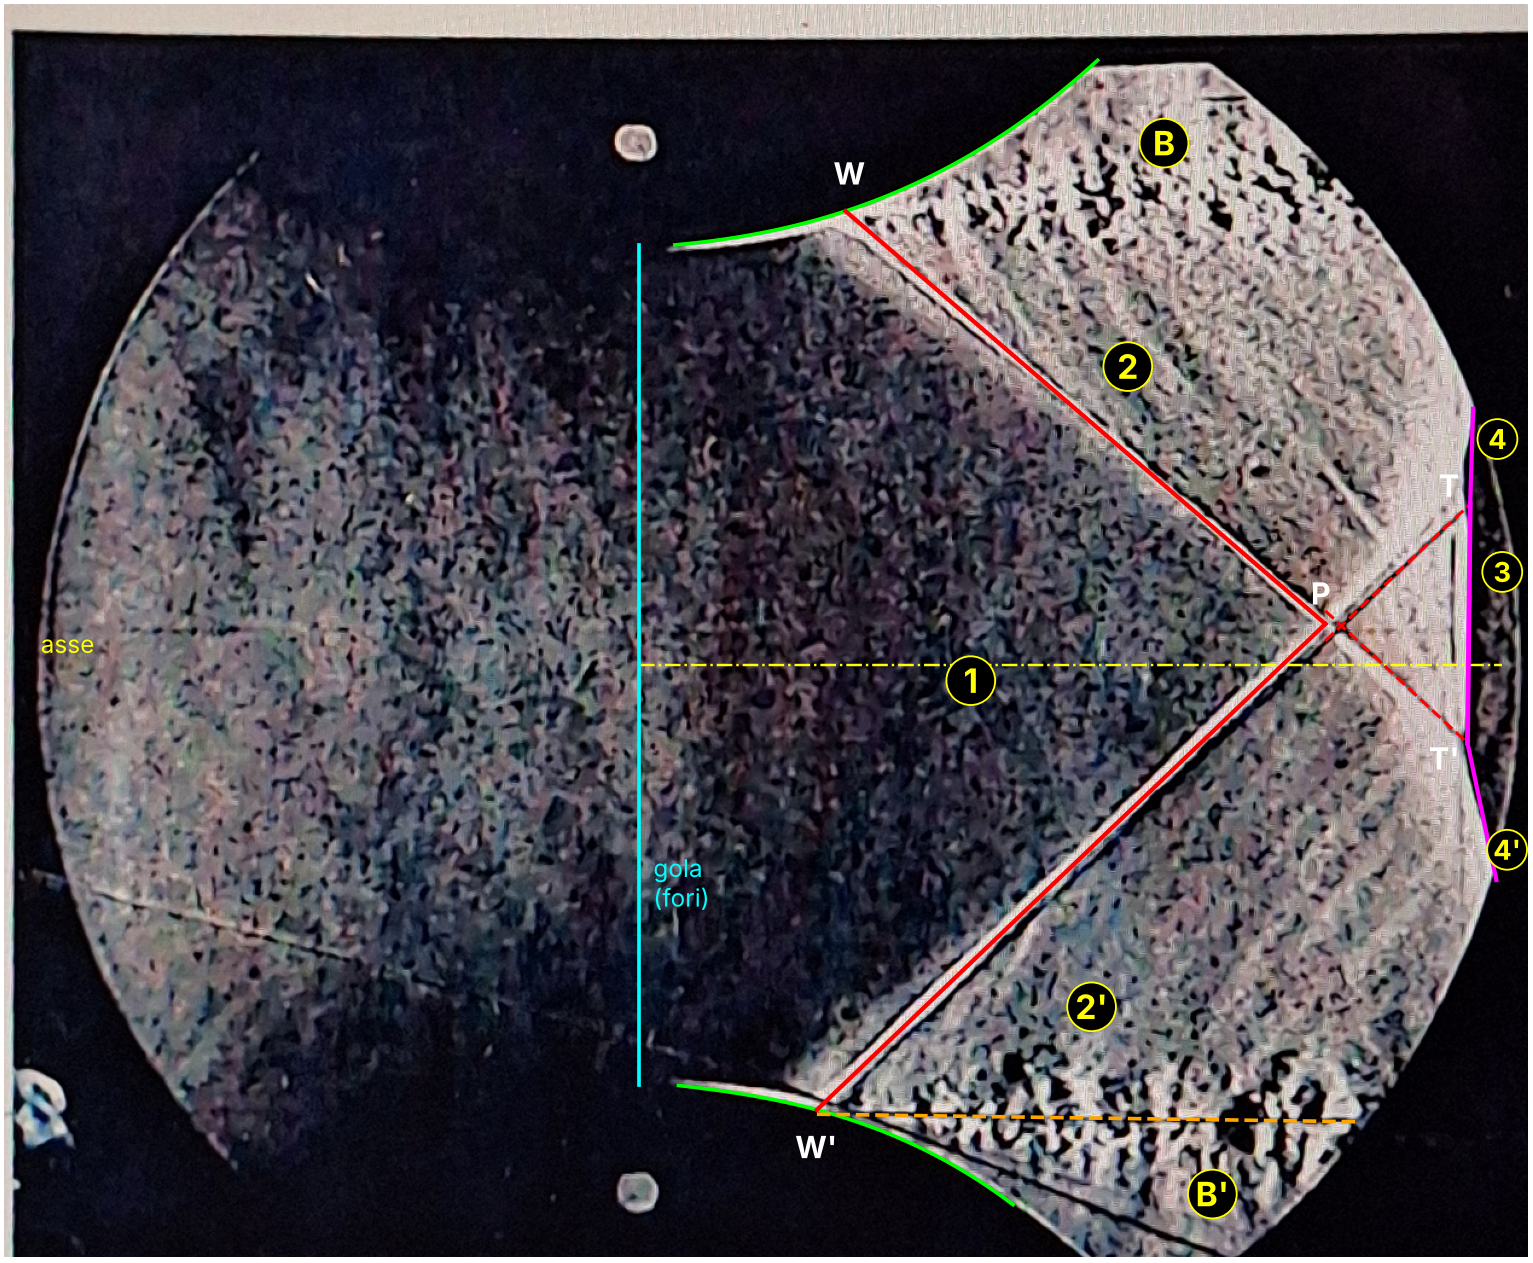
\includegraphics[width=0.64\textwidth]{annotata.png}
  \caption{Schlieren con le strutture identificate. Ciano: gola; verde: pareti; rosso: urti di separazione da W e
  W$'$ e loro prosecuzione oltre l'incrocio P (tratteggio); arancio: strato separato inferiore; magenta: gambetto di
  Mach fra i punti tripli T e T$'$ e urti obliqui forti che ne partono. I numeri indicano gli stati.}
  \label{fig:ann}
\end{figure}

%==============================================================================
\section{Identificazione delle strutture}
Nell'ordine in cui le incontra la corrente (fig.~\ref{fig:ann}):
\begin{enumerate}
\item \textbf{Convergente e gola} (sinistra e centro): luminosità senza strutture nette; nella zona 1, scura, la
  corrente accelera attraverso $M=1$ ed espande lungo le pareti convesse del divergente.
\item \textbf{Linee sottili che partono dalle pareti in W e W$'$}, a circa $0{,}2\,h^*$ dalla gola, dove lo strato
  limite si separa: sono gli \textbf{urti di separazione}. Quello da W è della famiglia $\Cm$, quello da W$'$ della
  famiglia $\Cp$.
\item \textbf{Strati separati} che partono da W e W$'$ quasi paralleli all'asse. Quello inferiore è netto (linea con
  frangia irregolare dovuta ai vortici del mescolamento); fra lo strato e la parete, che continua ad aprirsi, ci sono
  le \textbf{zone separate} B e B$'$, ad aria quasi ferma.
\item \textbf{Incrocio P} delle due linee, vicino all'asse: oltre P ciascuna prosegue con la stessa inclinazione.
\item \textbf{Estremo destro della finestra} (fig.~\ref{fig:det}): le due linee, oltre P, finiscono su un tratto di urto quasi verticale a
  cavallo dell'asse, il \textbf{gambetto di Mach} (fra T e T$'$); nei due \textbf{punti tripli} T e T$'$ il fronte
  piega e prosegue verso le pareti come \textbf{urto obliquo forte}, che delimita la zona chiara. A valle del fronte
  (zone 3, 4, 4$'$, la sottile fascia scura prima del bordo della finestra) la luminosità cambia: è la corrente
  subsonica dietro gli urti forti.
\end{enumerate}
Sono invece artefatti la tessitura a macchie (grana della stampa e della foto) e la fascia chiara sottile che
accompagna le pareti.

%==============================================================================
\section{Ipotesi e modello}
\begin{itemize}
\item La linea sottile che parte dalla parete in corrispondenza della separazione dice tre cose: (a) la gola è
  \textbf{efficace} (strozzata); (b) nel divergente la corrente è \textbf{supersonica}, perché solo lì può esistere un
  urto obliquo; (c) la pressione all'uscita, fuori dalla figura, è abbastanza alta da provocare la
  \textbf{separazione dentro il condotto}: l'ugello è sovraespanso.
\item Fino agli urti la corrente è adiabatica e isentropica; la uso nel modello 2D stazionario supersonico (urti
  obliqui, onde di Mach). Le zone separate sono a pressione uniforme $p_B$.
\item \textbf{Linea sonica} (Sauer--Meyer). Con $\xi$ lungo l'asse, $\eta$ trasversale ($\eta=\pm1$ a parete) e
  $d=1/\sqrt{(\gamma+1)R}$:
  \[
  u=d\,\xi+\frac{(\gamma+1)d^2}{2}\eta^2,\qquad
  \xi_{\rm gola}=-\frac d6\eta^2,\qquad
  \xi_{\rm sonica}=-\frac{(\gamma+1)d}{2}\eta^2 .
  \]
  A parete ($\eta^2=1$) la linea sonica sta a $\xi=-1{,}2\,d$, prima della sezione di gola ($\xi=-d/6$); sull'asse
  sta a $\xi=0$, dopo di essa. Non è richiesta la sua posizione: conta la conseguenza, che $M$ \textbf{non è uniforme
  sulla sezione} e, a parità di ascissa, è più alto a parete che sull'asse.
\item Uso la metà inferiore per la separazione, dove lo strato separato è netto, e i valori medi delle due metà per le
  strutture vicino all'asse.
\end{itemize}

%==============================================================================
\section{Misure sull'immagine}
\begin{minipage}[t]{0.68\textwidth}
\vspace{0pt}
Con righello e goniometro, prendendo l'asse come la mezzeria fra le due pareti:
\begin{itemize}
\item separazione inferiore W$'$ a $x\approx0{,}21\,h^*$, dove la parete è inclinata di \ang{-15}; strato separato a
  circa \ang{-1} sull'asse, cioè \textbf{\ang{14} rispetto alla tangente alla parete};
\item urto di separazione a circa \textbf{\ang{59} rispetto alla tangente alla parete}, su entrambi i lati;
\item vicino all'asse: urto da W$'$ inclinato di \ang{44} prima di P e di \ang{43} dopo; quello da W di \ang{41} e
  \ang{43}. In media \textbf{\ang{43}}, uguale prima e dopo l'incrocio;
\item gambetto di Mach a $x\approx0{,}99\,h^*$, perpendicolare all'asse;
\item urti obliqui forti dai punti tripli: \ang{81} da T e \ang{76} da T$'$ sull'asse, in media \textbf{\ang{79}}.
\end{itemize}
\end{minipage}\hfill
\begin{minipage}[t]{0.27\textwidth}
\vspace{0pt}
\centering
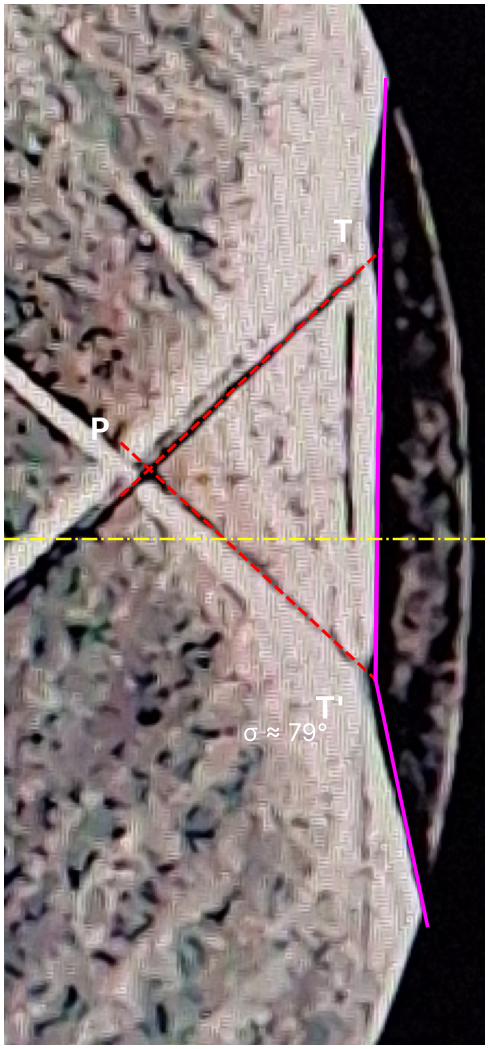
\includegraphics[width=\textwidth]{dettaglio_T.png}

\captionof{figure}{Estremo destro: incrocio P, gambetto di Mach T--T$'$, urti forti.}
\label{fig:det}
\end{minipage}

%==============================================================================
\section{Analisi qualitativa e topologia}
\begin{figure}[H]
  \centering
  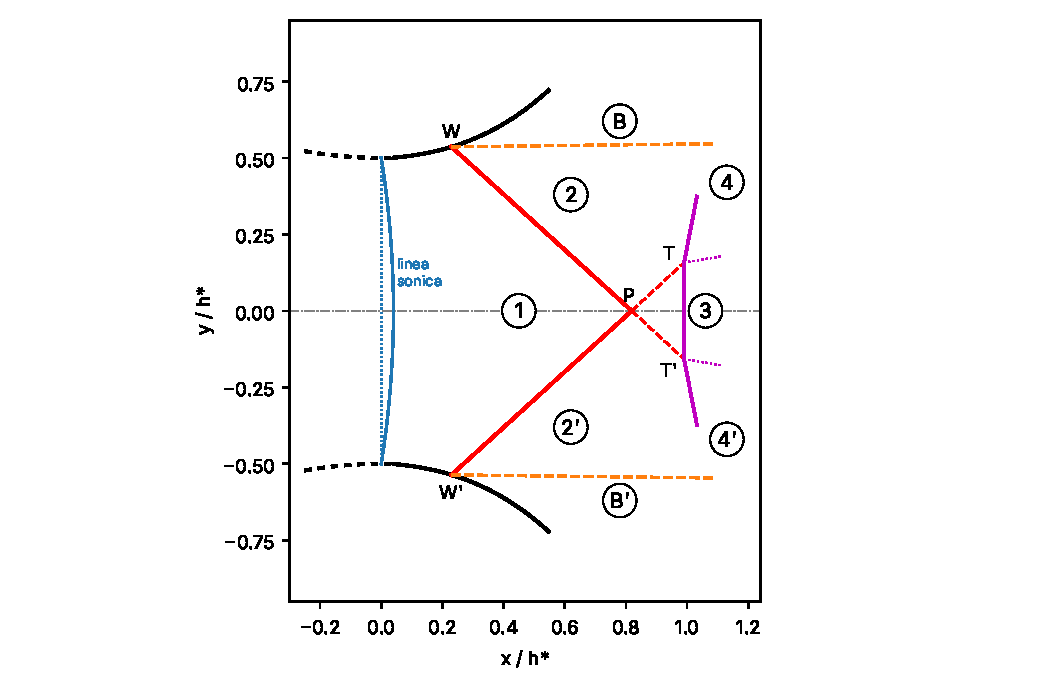
\includegraphics[width=0.66\textwidth]{schema.pdf}
  \caption{Schema del campo in unità di $h^*$: pareti misurate (tratteggio: convergente), linea sonica qualitativa,
  urti di separazione e loro prosecuzione oltre P, gambetto di Mach T--T$'$ e urti forti (magenta), linee di
  scorrimento dai punti tripli (punteggiato), strati separati (arancio).}
  \label{fig:schema}
\end{figure}
Le pareti convesse espandono la corrente a partire dalla linea sonica; l'espansione è più rapida vicino alle pareti,
quindi il nucleo 1 ha $M$ crescente verso valle e verso le pareti. L'urto di separazione nasce forte a parete (devia la
corrente di circa \ang{14}) e si indebolisce verso l'asse, dove arriva come un'onda quasi di Mach: per questo dopo
l'incrocio in P la direzione non cambia e il nucleo resta, sull'asse, nello stato 1. Al termine della zona visibile la
compressione richiesta dalla contropressione avviene con un urto quasi normale (gambetto di Mach), raccordato agli urti
obliqui forti nei punti tripli; dietro di essi la corrente è subsonica.

\begin{table}[H]
  \centering
  \small
  \begin{tabular}{cp{6.4cm}p{5.6cm}}
    \toprule
    Stato & Posizione & Come lo si raggiunge \\
    \midrule
    1 & nucleo supersonico fra gola e urti (1$_W$ a parete prima di W$'$; sull'asse prima di T) & espansione
    isentropica \\
    2, 2$'$ & dietro gli urti di separazione, lungo gli strati separati & urto di separazione \\
    B, B$'$ & zone separate a parete, $p=p_B$ & strato separato \\
    3 & dietro il gambetto di Mach, sull'asse & urto normale \\
    4, 4$'$ & dietro gli urti forti che partono da T, T$'$ & urto obliquo forte \\
    \bottomrule
  \end{tabular}
  \caption{Stati. Fra 3 e 4 (e fra 3 e 4$'$) c'è la linea di scorrimento che parte dal punto triplo.}
\end{table}

%==============================================================================
\section{Calcolo}

\subsection*{a) Separazione: $M$ a parete a monte di W$'$ (1$_W\to$2$'$)}
Deviazione $\theta=\ang{14}$ (strato separato rispetto alla parete) e angolo d'urto $\sigma=\ang{59}$ (rispetto alla
stessa direzione, che è quella della corrente a monte). Invertendo la relazione $\theta$--$\sigma$--$M$:
\[
M_1^2=\frac{2(\tan\theta+\cot\sigma)}{2\cot\sigma\sin^2\sigma-\tan\theta\,(\gamma+\cos2\sigma)}
=\frac{2(0{,}249+0{,}601)}{2\cdot0{,}601\cdot0{,}735-0{,}249\,(1{,}4-0{,}469)}=\frac{1{,}700}{0{,}651},
\]
quindi $M_1\approx1{,}62$,
con $p_1/p_0=(1+0{,}2\cdot1{,}62^2)^{-3{,}5}=0{,}228$. Dietro l'urto:
\[
M_{n1}=1{,}62\sin\ang{59}=1{,}39,\qquad \frac{p_2}{p_1}=1+\frac{2\gamma}{\gamma+1}(M_{n1}^2-1)=2{,}08,
\]
\[
M_{n2}^2=\frac{1+0{,}2M_{n1}^2}{1{,}4M_{n1}^2-0{,}2}\ \Rightarrow\ M_{n2}=0{,}745,
\]
\[
M_2=\frac{M_{n2}}{\sin(\sigma-\theta)}=\frac{0{,}745}{\sin\ang{45}}\approx1{,}05,\qquad
\frac{p_B}{p_0}\simeq\frac{p_2}{p_0}=2{,}08\cdot0{,}228\approx0{,}47 .
\]

\subsection*{b) Asse: onda di Mach in P}
Vicino all'asse l'urto arriva inclinato di circa \ang{43} e, oltre l'incrocio, prosegue con la stessa inclinazione:
un urto di intensità finita, dopo l'incrocio, cambierebbe inclinazione perché attraversa una corrente già deviata. È
quindi un'\textbf{onda di Mach} del nucleo, e il suo angolo è l'angolo di Mach:
\[
M=\frac{1}{\sin\mu}=\frac{1}{\sin\ang{43}}\approx1{,}47,\qquad \frac{p}{p_0}=(1+0{,}2\cdot1{,}47^2)^{-3{,}5}=0{,}284 .
\]
Il valore sull'asse, pur letto più a valle, è minore di quello a parete prima della separazione, come prevede
Sauer--Meyer.

\subsection*{c) Punto triplo: gambetto di Mach e urto obliquo forte}
Per semplicità prendo a monte di T$'$ (e di T) lo stato 1 dell'asse: $M_1=1{,}47$, corrente parallela all'asse.
\begin{itemize}
\item \textbf{Gambetto di Mach} (urto normale, 1$\to$3):
\[
\frac{p_3}{p_1}=1+1{,}167\,(1{,}47^2-1)=2{,}35,\qquad M_3^2=\frac{1+0{,}2\cdot1{,}47^2}{1{,}4\cdot1{,}47^2-0{,}2}
\Rightarrow M_3=0{,}71,\qquad \frac{p_3}{p_0}=0{,}67 .
\]
\item \textbf{Urto obliquo forte} con $\sigma=\ang{79}$ (1$\to$4$'$):
\[
M_{n1}=1{,}47\sin\ang{79}=1{,}44,
\]
\[
\tan\theta=2\cot\sigma\,\frac{M_1^2\sin^2\sigma-1}{M_1^2(\gamma+\cos2\sigma)+2}=\frac{0{,}421}{3{,}02}=0{,}139
\ \Rightarrow\ \theta\approx\ang{8},
\]
\[
\frac{p_4}{p_1}=2{,}26,\qquad M_{n2}=0{,}722,\qquad M_4=\frac{0{,}722}{\sin(\ang{79}-\ang{7.9})}\approx0{,}76,\qquad
\frac{p_4}{p_0}=0{,}64 .
\]
La corrente ruota di circa \ang{8} allontanandosi dall'asse.
\end{itemize}

%==============================================================================
\section{Verifiche}
\begin{enumerate}
\item $M$ a parete prima della separazione con l'onda semplice ($\nu=|\theta_w|=\ang{14.9}$): $M=1{,}60$, contro
  $1{,}62$ dalla relazione $\theta$--$\sigma$--$M$. \emph{Verificata.}
\item Urto di separazione sul ramo debole: $\theta=\ang{14}<\theta_{\max}(1{,}62)=\ang{15.1}$ e
  $\sigma=\ang{59}<\ang{65.7}$ (angolo del punto di $\theta_{\max}$); $M_2\approx1{,}05$, appena supersonico.
  \emph{Verificata, ma vicino al distacco.}
\item Onda in P: stessa inclinazione prima e dopo l'incrocio (\ang{44} e \ang{43} per quella da W$'$). \emph{Coerente con
  un'onda di Mach.}
\item Ordine dei valori: $M$ a parete ($1{,}62$ a $0{,}21\,h^*$) maggiore di $M$ sull'asse ($1{,}47$ a $0{,}8$--$1\,h^*$).
  \emph{Coerente con Sauer--Meyer.}
\item Urto forte: $\sigma=\ang{79}$ maggiore dell'angolo del punto di $\theta_{\max}(1{,}47)$ (\ang{66.9}), e
  $\theta=\ang{8}<\theta_{\max}=\ang{11.3}$: ramo forte, $M_4<1$. \emph{Verificata.}
\item Separazione: $p_1/p_B=0{,}228/0{,}47=0{,}48$, nell'ordine dei valori tipici della separazione negli ugelli
  (circa 0,4). \emph{Coerente.}
\end{enumerate}

%==============================================================================
\section{Risultati}
\begin{table}[H]
  \centering
  \begin{tabular}{lll}
    \toprule
    Posizione & $M$ & $p/p_0$ \\
    \midrule
    linea sonica (a parete prima della gola, sull'asse dopo) & 1 & 0,528 \\
    parete, fino alla separazione ($x\approx0{,}21\,h^*$) & fino a $\approx1{,}62$ & fino a 0,228 \\
    asse, da P al gambetto ($x\approx0{,}8$--$1\,h^*$) & $\approx1{,}47$ & 0,284 \\
    dietro l'urto di separazione (2, 2$'$) & $\approx1{,}05$ & $\approx0{,}47$ \\
    zone separate (B, B$'$) & $\approx0$ & $\approx0{,}47$ \\
    dietro il gambetto di Mach (3) & $\approx0{,}71$ & 0,67 \\
    dietro gli urti forti (4, 4$'$), $\theta\approx\ang{8}$ & $\approx0{,}76$ & 0,64 \\
    \bottomrule
  \end{tabular}
\end{table}

%==============================================================================
\section{Rappresentazioni}
\begin{figure}[H]
  \centering
  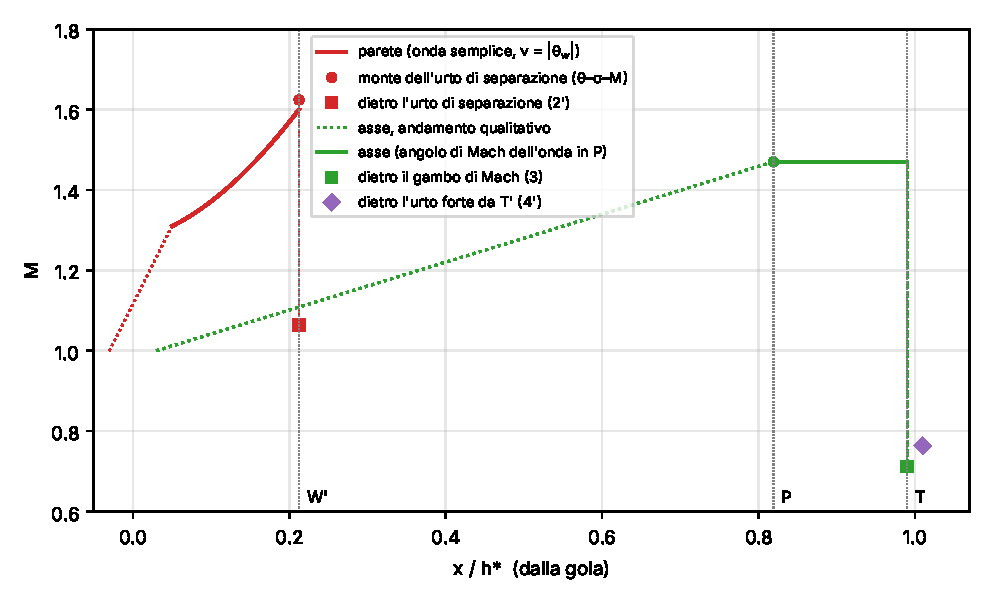
\includegraphics[width=0.72\textwidth]{mach.pdf}
  \caption{Distribuzione di $M$ a valle della gola, a parete e sull'asse, con i valori dietro gli urti.}
  \label{fig:mach}
\end{figure}
\textbf{Distribuzione di $M$} (fig.~\ref{fig:mach}). A parete $M$ parte da 1 poco prima della gola e cresce
rapidamente lungo la parete convessa (curva dall'onda semplice, $\nu=|\theta_w|$, con le inclinazioni misurate) fino a
1,62 alla separazione, dove scende a circa 1,05 attraverso l'urto. Sull'asse $M$ vale 1 poco dopo la gola e cresce più
lentamente (tratto punteggiato: solo qualitativo) fino a 1,47 in P; resta tale fino al gambetto di Mach, dove scende a
0,71. Il punto viola è la corrente dietro l'urto forte.

\begin{figure}[H]
  \centering
  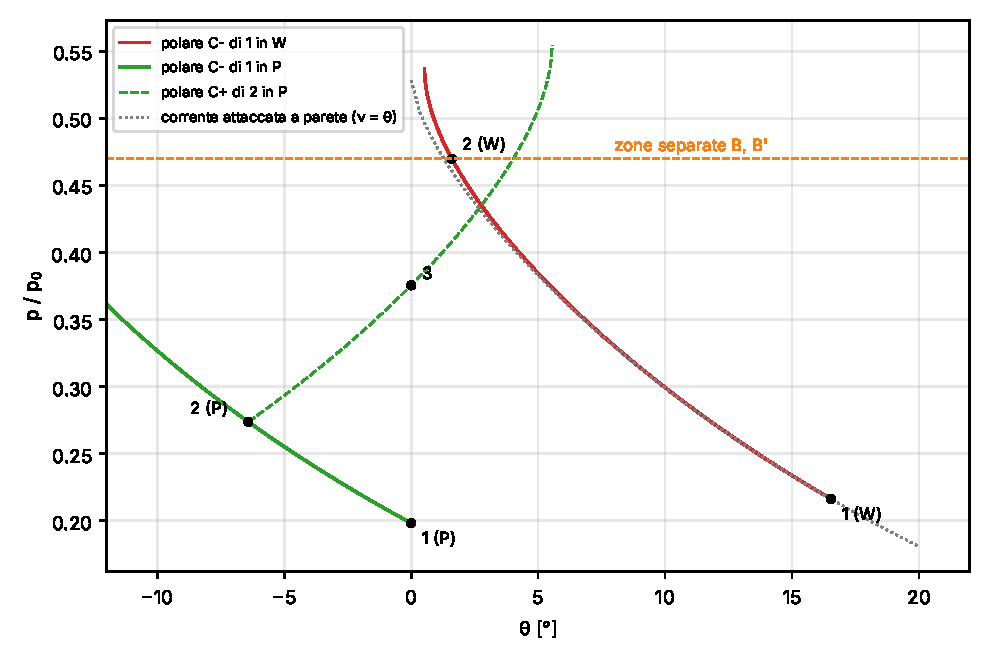
\includegraphics[width=0.68\textwidth]{p_theta.pdf}
  \caption{Piano $p$--$\theta$ per la metà inferiore (pressione riferita a $p_0$).}
  \label{fig:pth}
\end{figure}
\textbf{Piano $p$--$\theta$} (fig.~\ref{fig:pth}). La curva punteggiata è la corrente attaccata lungo la parete
inferiore, che arriva in 1$_W$ ($\theta=\ang{-15}$). La polare $\Cp$ di 1$_W$ porta, sul ramo debole e vicino al suo
massimo, a 2$'$ ($\theta\approx\ang{-1}$), sulla retta $p=p_B$ delle zone separate. Sull'asse la polare $\Cm$ dello stato 1
contiene sia il gambetto di Mach (3, in cima, $\theta=0$) sia l'urto forte (4$'$, $\theta\approx\ang{-8}$): entrambi
sul ramo forte, molto sopra $p_B$. Le pressioni stanno fra $0{,}23\,p_0$ e $0{,}67\,p_0$, quindi basta la scala
lineare.

%==============================================================================
\section{Coerenza con l'immagine e discussione}
\begin{itemize}
\item Il modello ritrova le strutture visibili: urti di separazione con l'angolo misurato, strato separato quasi
  parallelo all'asse ($\theta_2\approx\ang{-1}$, come misurato), onde che attraversano l'asse senza cambiare
  inclinazione, fronte quasi normale vicino all'asse che piega di circa \ang{11} nei punti tripli.
\item L'urto di separazione è rettilineo ma la sua intensità non è costante: a parete forma \ang{59} con la corrente
  ($M_{n1}=1{,}39$), sull'asse \ang{43}, cioè l'angolo di Mach. La differenza viene dal nucleo non uniforme: verso
  l'asse $M$ è più basso e la corrente è parallela all'asse.
\item Il punto triplo qui è degenere: l'onda che vi arriva è di Mach, quindi gambetto e urto forte sono lo stesso fronte,
  quasi normale vicino all'asse e inclinato più all'esterno. Le pressioni dietro i due tratti (0,67 e $0{,}64\,p_0$)
  differiscono di poco; l'equilibrio attraverso la linea di scorrimento lo realizza la curvatura del gambetto,
  trascurata assumendolo normale.
\item Dietro il fronte la corrente è subsonica e a pressione maggiore di $p_B$: a valle, fuori dalla figura, riaccelera
  verso l'uscita. La stima più sensibile alle misure è quella dell'urto forte: per $M_1=1{,}47$ la deviazione varia di
  circa mezzo grado per ogni grado di $\sigma$, quindi $\theta\approx\ang{8}$ è indicativo.
\end{itemize}

\end{document}
